\documentclass[12pt]{article}

%\usepackage{times} %for Times New Roman, if required
\usepackage[top=1in, bottom=1in, left=1in, right=1in]{geometry} %adjust margins. TODO: hack to fix large top margin
\usepackage{setspace} %allows doublespacing, onehalfspacing, singlespacing
\usepackage{enumitem} %for continuing lists
\usepackage{titling} %for moving the title
\usepackage[normalem]{ulem} %for underlining
\usepackage{graphics}

\begin{document}

\begin{spacing}{.4}
\setlength{\droptitle}{-7em}
\title{CSE 485 Project Initialization \\ Team 1, Friday 10:30am}
\author{Connor Alfheim \and Ryan Dougherty \and David Ganey \and Dylan Lusi \and Joseph North \and Ben Roos}
\maketitle
\newpage
\end{spacing}

\begin{spacing}{1.5}

\section*{Table of Contents}
\begin{enumerate}
\item Overview
\item Requirements
\item First Semester Plan
\item Conclusion
\end{enumerate}
\newpage

\section{Overview}
\subsection{Introduction}
The Murchison Widefield Array is a radio telescope being used to measure hydrogen in space with the goal of obtaining a better understanding of how stars form. This type of telescope comes with some significant engineering problems: firstly, it involves the coordination of dozens of independent computer systems, and secondly, it generates petabytes of complex data yearly that requires intensive processing. The end result is a situation unfamiliar to the field of astronomy. What this situation requires is a system that enables the monitoring of the telescope and the orchestration of data flow, metadata searching, and data processing commands within a unified interface. That is the goal of this project: to create a platform that allows astrophysicists and cosmologists to extract more meaning out of the data they have so they can make sense of it.

\subsection{Description}
The project involves all the major components of a modern Web application. The foundation of the application will be on Amazon Web Services, specifically the Elastic Compute Cloud (EC2) Platform as a Service. On this server framework, MySQL will handle the database operations. Python will likely be used for some data processing scripts, and standard Web tools (e.g. HTML, JavaScript) will be used to handle the front end. While not all the technology choices have been made yet, it is clear the project will involve the entire stack.
\newline \newline
As important as the functional Web application is the ability to easily extend it. As this capstone project is limited in scope to just two semesters, the necessary exodus of 100\% of the project's developers will necessitate modifications down the road by others. Since the application will primarily be used by astrophysicists, it is important that it be modifiable without a significant software development background. This will be done in multiple ways. Clean, well-written code, efficient segregation of interfaces, and minimal interdependencies will make the code easy to understand. A comprehensive version control history will make modifications easier to trace. Ultimately, the most important method of achieving future extensibility will be a simple ORM (object-relational mapping) schema and database API which should allow scientists to "plug in" custom data modules and allow them to appear on the website.

\subsection{Assumptions}
No significant assumptions will be required for this project. Because the project involves improving an existing system, we are able to know how the system will be used and tailor the performance to those situations. If assumptions become necessary during the course of development, they will be made known to the project sponsors.

\newpage

\section{Requirements}
The Web system has the following requirements:
\begin{enumerate}
\item The Web application should display the current status of the Murchison Widefield Array. The application should display the status of the array in a visual format.
\item The application will support user accounts.
	\begin{enumerate}
	\item Signing in will be required to act on the website, but not to read it.
	\item Users should be able to customize their experience by subscribing to various feeds, modules, etc.
	\item Users can create accounts only with permission from a site admin.
	\end{enumerate}
\item The application should support some data processing. Data collected in periods during which the MWA had malfunctioning nodes should be flagged.
\item The team should generate an API which allows astronomers with limited knowledge of software development to add, extend, and modify the application functionality.
\end{enumerate}

\subsection{Deliverables}
The team will deliver a functional website running on an EC2 instance. The team will be agile, so as the requirements change, so will the specifics of the delivered website. Documentation to maintain future extensibility after the conclusion of the project will accompany the web platform.

\subsection{Use-case diagrams}
The use-cases for the website are fairly straightforward. Since the application is primarily a data viewer and status monitor, most use-cases simply involve observing data.
\subsubsection{Figure 1: User with account}
\begin{center}
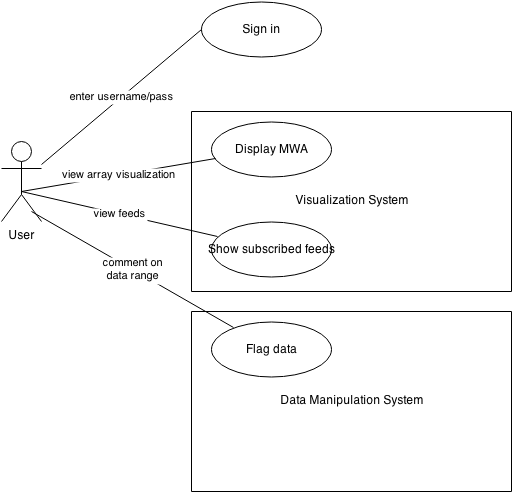
\includegraphics{usecase1} %we can use this to insert .png files in the same directory
\end{center}
\newpage
Users who are not logged in are not permitted to edit the data:
\subsubsection{Figure 2: User without account}
\begin{center}
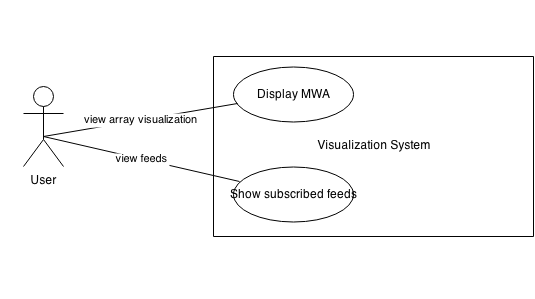
\includegraphics{usecase2}
\end{center}

\subsection{User stories}
\begin{enumerate}
\item User views website
	\begin{itemize}
		\item As a user who is not signed in, I should see a graphical representation of the Murchison Widefield Array. This visualization should make it clear if any nodes are malfunctioning.
		\item Given that the data stream is valid, when the user loads the page, the page should show a graphic which shows the state of the array
	\end{itemize}
\item User signs in
	\begin{itemize}
        		\item As as user with an account, I should be able to sign in to a persistent account on the server.
        		\item Given that the user credentials are valid, the website should allow the user to sign in and should load their personal settings before rendering the page
		\item Given that the user credentials are invalid, the website should refuse to allow the user to sign in but should still show the status of the array
	\end{itemize}
\item User modifies settings
	\begin{itemize}
		\item As a user, I should be able to modify my subscription settings after signing in.
		\item I should be able to choose which data streams I can see.
		\item Given that the user is properly signed in, the user should be permitted to modify subscription settings
		\item Given that the user is not properly signed in, the user should not be permitted to see or modify subscription settings
	\end{itemize}
\item User flags data
	\begin{itemize}
		\item As a user, I should be able to leave comments on data streams after signing in. The comments should contain information such as username and date in addition to the user's text.
		\item Given that the user is properly signed in, and that the data stream is valid, the user should be permitted to leave comments on a data stream.
		\item Given that the user is not properly signed in or that the data stream is not valid, the user should not be permitted to leave comments on that data stream.
	\end{itemize}
\end{enumerate}

\subsection{Non-functional requirements}
The primary goal of the project is \emph{extensibility}. The API developed by the team should allow individuals who are not software developers to modify and add functionality to the website. As a result, scalability and long-term maintainability are significant nonfunctional requirements. Additionally, standard constraints on security and efficiency apply. The website should not be vulnerable to standard exploits (e.g. no passwords stored in plaintext), and should scale appropriately to deliver a pleasant experience to all users.

\newpage

\section{First Semester Plan}
During the first semester, the team members will distribute themselves among several subteams corresponding to different areas of focus: the database, the front end, and the extensibility API. All members should be functional in all areas, but the sponsors and the team agree that some team members will specialize in specific areas (e.g. the database). After the subteams have been determined, the database team will meet with the sponsors to discuss the database schema. Due to the complexity of the database, a small portion of it will be copied to our test instance to be used in testing.
\newline \newline
Once the EC2 instance is up and running with the database, the team will clone the existing code repository to use it as a base. Whether any of the current code remains in the website is a decision the team will make after reviewing the source code itself. The team will then begin to build features. It is likely that the basic user account functionality will be built first, followed by the primary visualization dashboards with a focus on the telescope status monitor.

\subsection{Initial scope}
The initial goal of the project is to build the framework for the website. Once user functionality is enabled, different view modules will be added. Throughout the project, the team will make easy extensibility a high priority.

\subsection{Milestones}
\subsubsection{Table 1: First Semester Schedule}
\begin{tabular}{l | l}
Date			&	Goal \\
\hline
10/7/2014		&	Project Initialization form sent to sponsors \\
\hline
10/10/2014		&	Project Initialization form complete \\
\hline
10/20/2014		&	Database copy completed \\
\hline
11/15/2014		&	Basic user functionality implemented \\
\hline
12/5/2014		&	Basic telescope visualizer implemented \\
\hline
12/5/2014		&	Classes end \\
\end{tabular}

\newpage

\section{Conclusion}
For this project, we need to create a platform that integrates the metadata describing the operational status of the Murchison Widefield Array with the data  of interest to astrophysicists that it collects. Any information relating to faults with the equipment is critical to the meaning of the data collected during the faulty period, and our solution needs to provide a means to tie these data together so the users of the data can make smarter decisions. Not only should a user of our system be able to monitor the status of the telescope in real time, he should also be able to view customizable data modules that extract meaning from the petabytes of data generated by the telescope. Ultimately, we need to construct a ``virtual observatory'' that is designed with hands-on astrophysicists and cosmologists in mind.

\end{spacing}
\end{document}

